\chapter{Implementation}
\label{ch:implementation}
\section{Introduction}
This chapter describes the planning and implementation phases. Software development methodologies are reviewed and discussed. Then, the planning steps for the project are outlined. Finally, the implementation process of the project is documented, and challenges faced during the phase are discussed and analysed.

\section{Software Development Methodology}
There are a number of methodologies we can follow to develop this system \cite{sdlc2010}, each with its own advantages in certain use cases. It is important to consider the relatively short time frame for this project, especially with the fixed deadline. Furthermore, we have already established an initial requirements specification based on user feedback. This section reviews several development models, and justifies the selected model for this system.

\subsection{Waterfall Model}
The waterfall model \cite{royce1987managing} is characterised by its distinct phase design, starting with evaluation and ending with deployment, where one phase follows the other sequentially. The basic model is shown in Figure~\ref{fig:waterfall}, but there have been iterations of the model by \citet{royce1987managing} which provide feedback loops between the phases.

This design works well where the requirements can be established at the start of the project, which would be effective in this project. However, it does not cope well when there are complications in later phases which can cause time delays; nor does it cope well when requirements are not yet known or may change throughout the process \cite{sdlc2010}.

	\begin{figure}
		\centering
		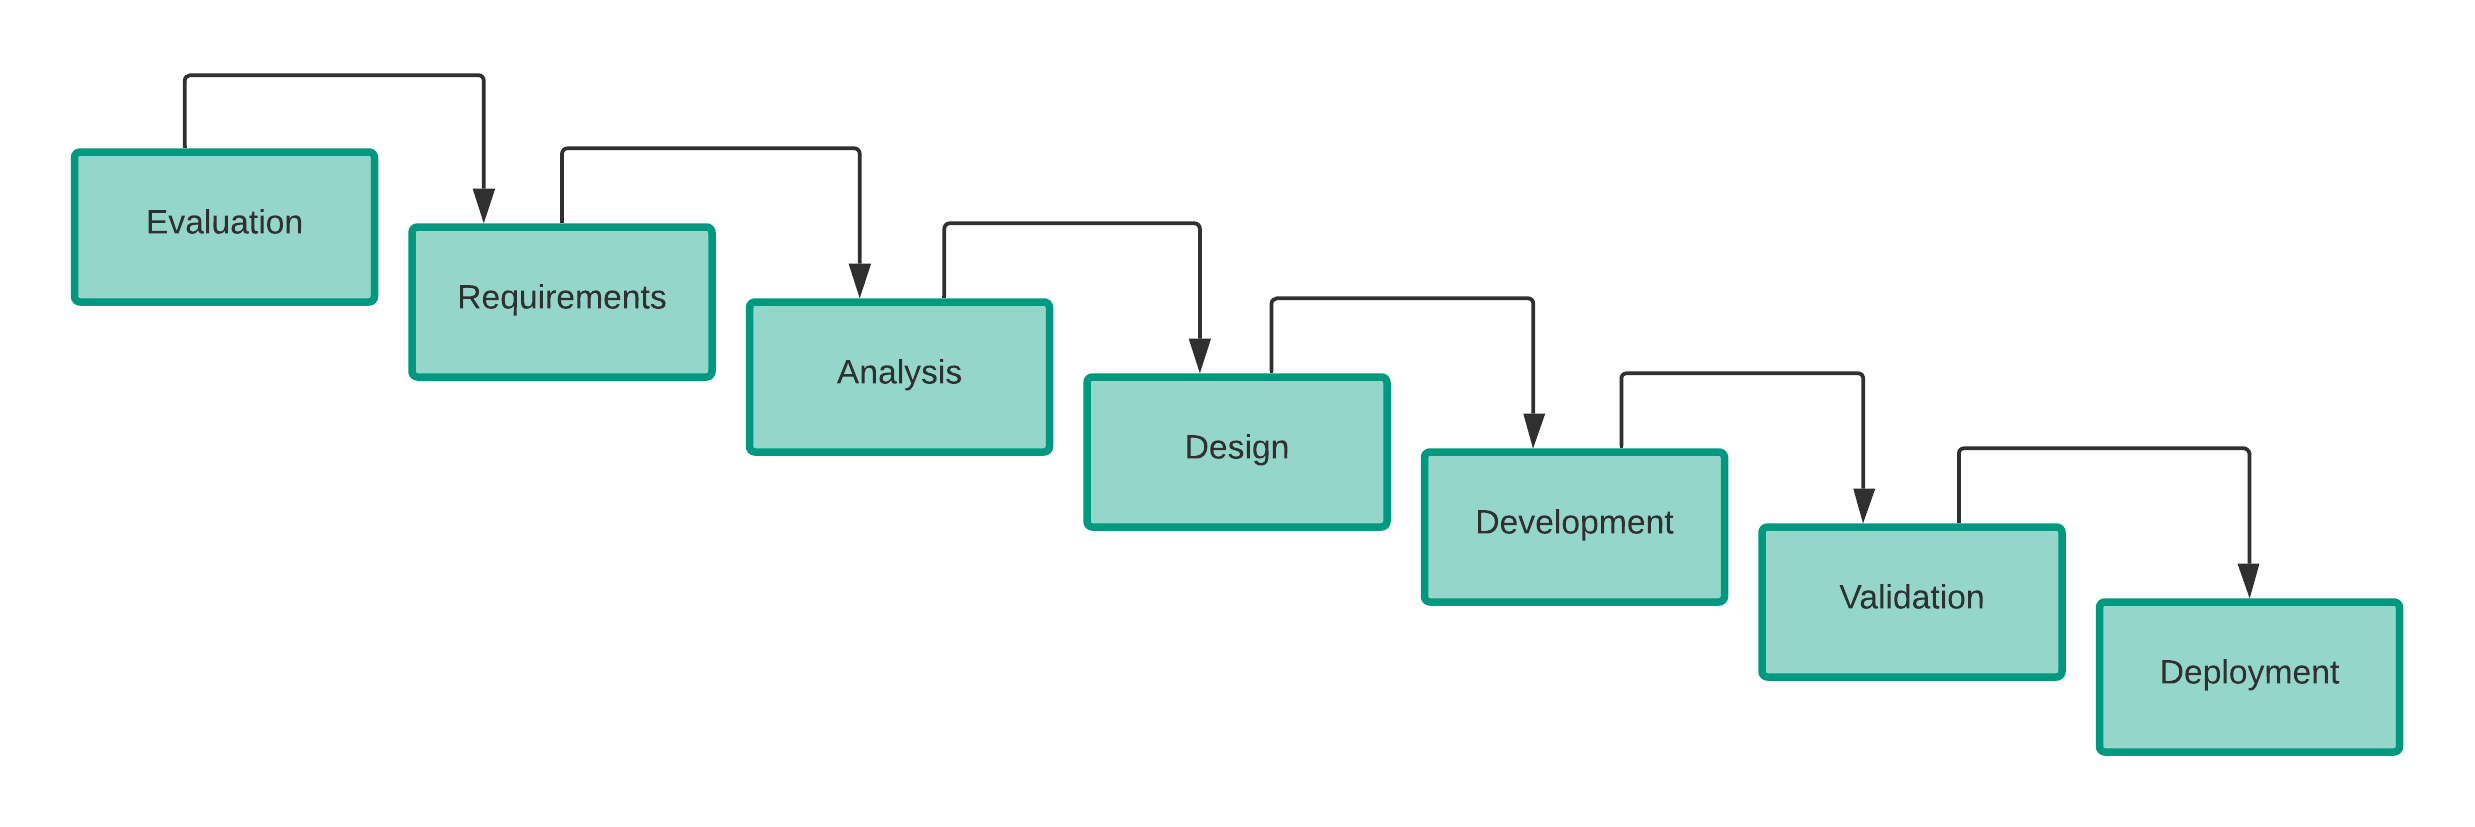
\includegraphics[width=0.8\linewidth]{waterfall}
		\caption{Waterfall model \cite{sdlc2010}}
		\label{fig:waterfall}
	\end{figure}

\subsection{V-Model}
\hilight{continue}
\begin{figure}
	\centering
	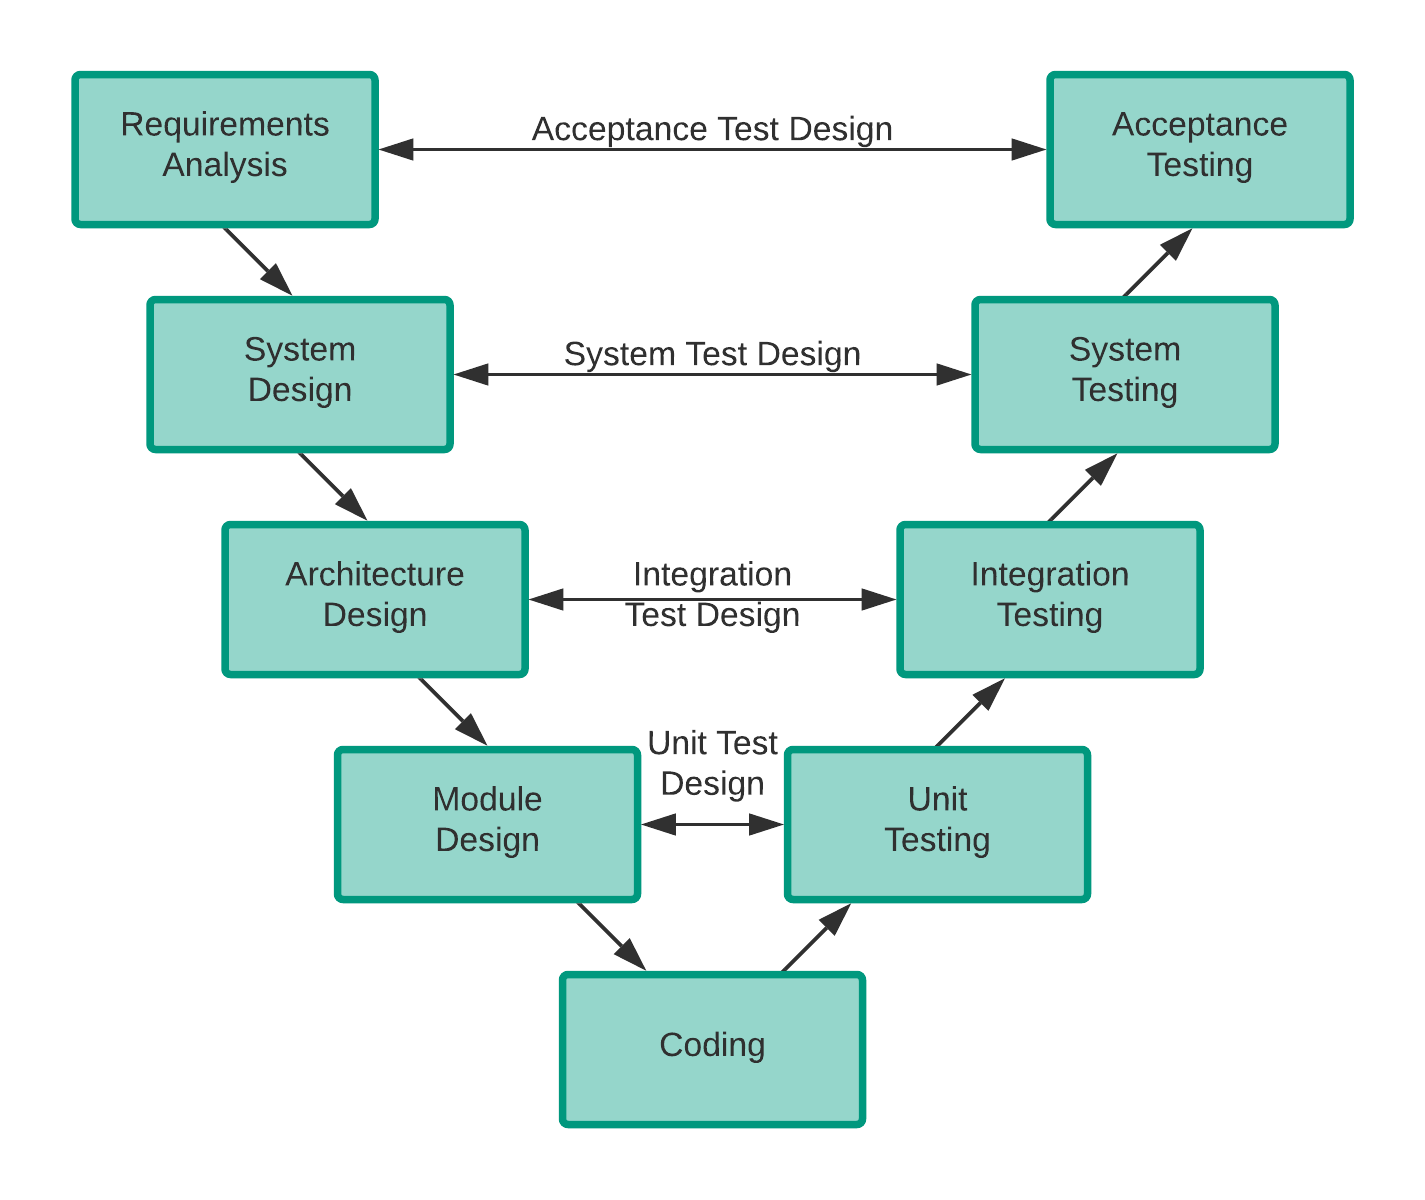
\includegraphics[width=0.6\linewidth]{vmodel}
	\caption{V-Model}
	\label{fig:vmodel}
\end{figure}

\subsection{Spiral Model}
\hilight{continue}
	\begin{figure}
	\centering
	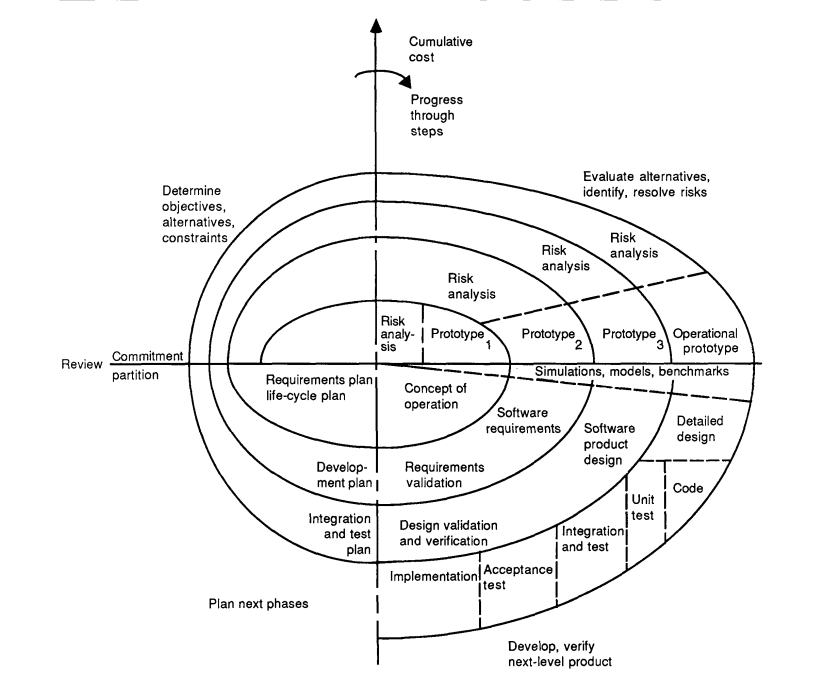
\includegraphics[width=0.6\linewidth]{spiral}
	\caption{Spiral Model}
	\label{fig:spiral}
\end{figure}

\subsection{Chosen Methodology}
There are many methodologies not explored in this section, such as Agile, which are effective in environments with multiple team members \cite{agile}. In this project, we will be using the V-Model. This is because having distinct phases will allow for logical planning steps. It shares similarities with the waterfall model, but divides the testing and integration phases into manageable steps. Methodologies with continual user feedback, such as the spiral model, would be harder to implement because the test users for this project have other commitments, so waiting constant communication with them may delay the project.

\section{Planning}
As the timeline of the project is restricted and has a fixed deadline, it is important that the project is planned carefully in order to deliver a complete solution. To achieve this, a Gantt chart was produced as an effective method to visualise the tasks of the project, with associated time scales \cite{wilson2003gantt}. The completed Gantt chart is shown in Figure~\ref{fig:gantt} (note that this chart is taken from after the project was completed, where red slots are tasks which overran - this is discussed further in Chapter~\ref{ch:conclusion}). The tasks were divided in a logical manner, where the implementation tasks are associated with the functional requirements from the specification in Section~\ref{sec:requirements}. This proved to be an effective visual plan to ensure that the requirements were met in a timely manner.

\section{Version Control}
During this implementation phase, it is important to manage the source code and maintain a consistent code base. As new features are added to meet the requirements, a version control system can keep records of file changes, so that we can recall previous versions, as well as develop new features without effecting previous versions.

For this project, Git will be used because of its popularity and personal familiarity with the tool. Git allows for branching, which will be useful when implementing a new function, merging, and comments to allow for a maintainable repository.

\section{Dependency Management}
As the project will depend on a number of external libraries, it is important to manage these dependencies in a consistent and repeatable way. For this project, Apache Maven\footnote{https://maven.apache.org/} is used because of the high availability of the required repositories for this project, including Spring and Program AB. Maven also provides a number of tools for building and deploying the project, which becomes important during the testing phase when the project is deployed to an external web server.

\begin{landscape}
	\begin{figure}[h]
		\centering
		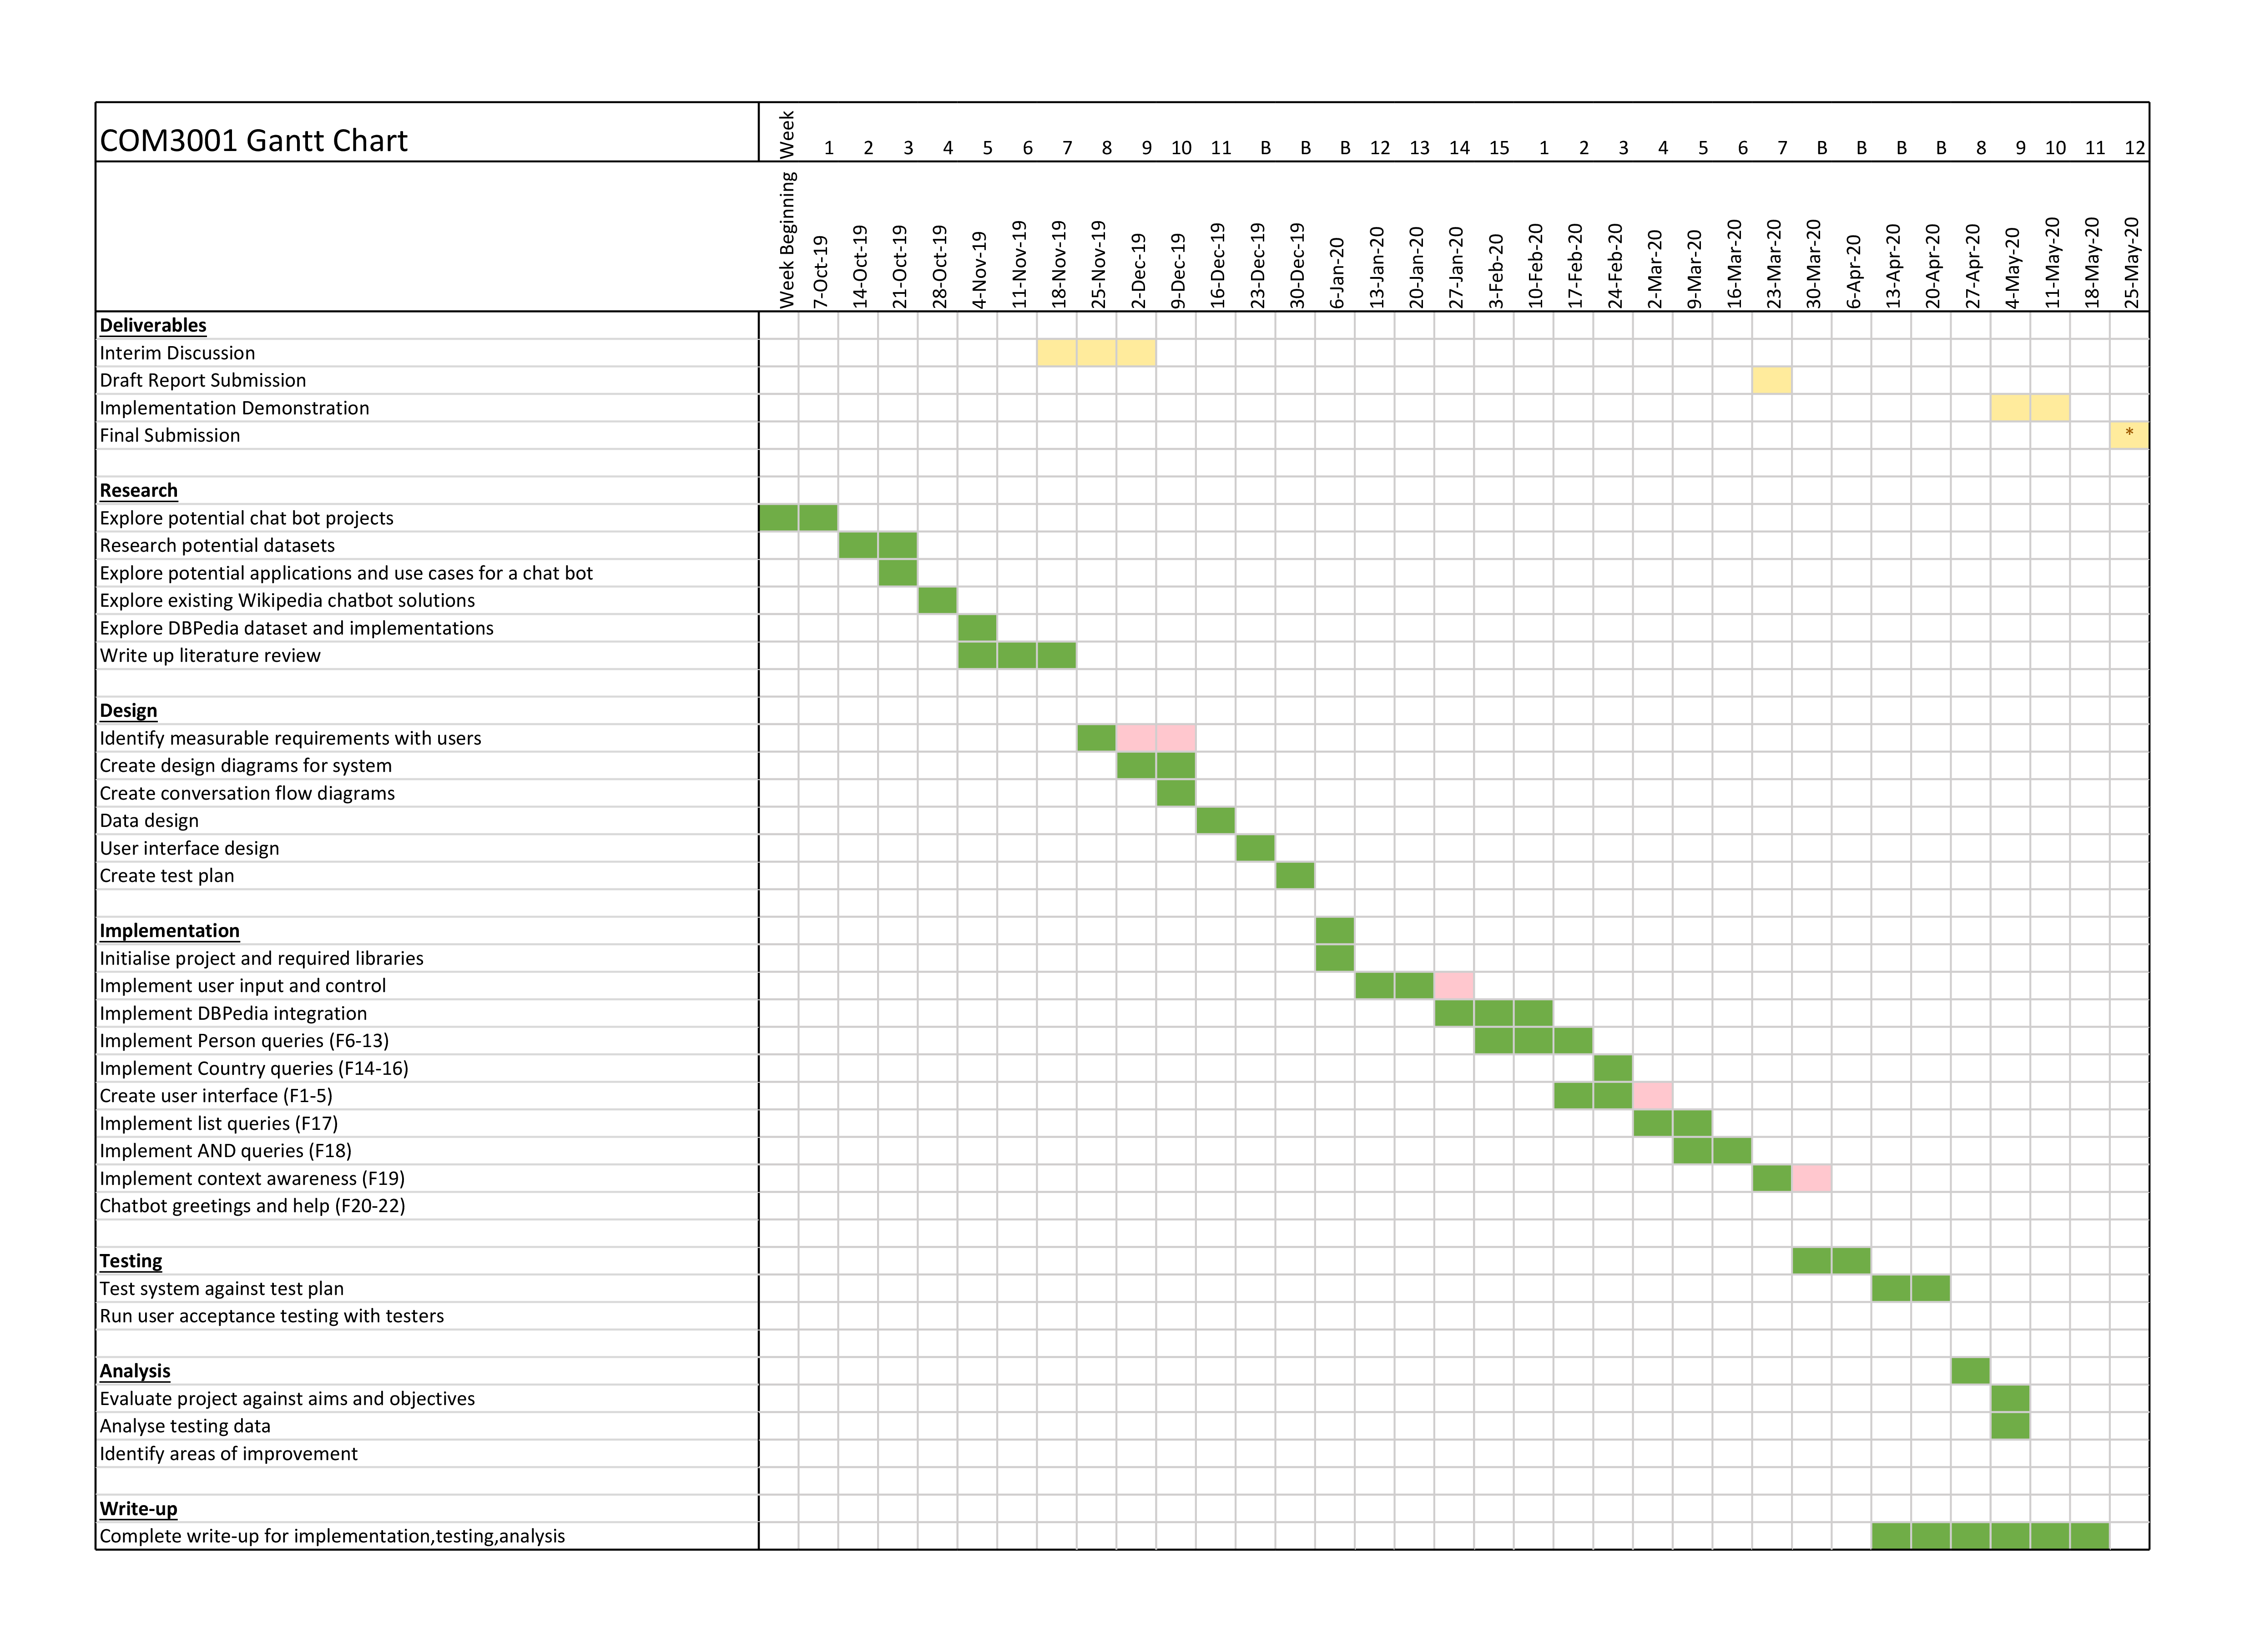
\includegraphics[width=0.9\hsize]{gantt}
		\caption{Gantt chart for planning}
		\label{fig:gantt}
	\end{figure}
\end{landscape}



\section{Implementation Process}
Following the Gantt chart and the development methodology, the implementation process was carried out iteratively. This section documents some of the key steps in the development process, how these were achieved, and gives some explanation to how the logic was created to meet the requirements of the system.

\subsection{Initialisation}
The first step of the implementation was to initialise a Git repository and a Java environment with Maven dependency management. Since the project would depend on many libraries for displaying and processing data, Maven is able to manage versioning and interdependencies of these libraries.

\subsection{Program AB}
As a result of the research in earlier phases, it was decided that this system would use a rule-based chatbot architecture, namely AIML as it is widely used in current chatbot systems. Program AB is a Java implementation of AIML 2.0 provided by ALICE A.I. Foundation \cite{programab_2013}. While this repository is no longer being developed, the choice for this project was to use a fork of this source, which is provided as a Maven dependency \cite{lumenrobot2016}.

Once the Maven dependency had been loaded into the project's \code{pom.xml} file, I was able to experiment with the chatbot. The \code{program-ab} source contains the original AIML implementation of a bot named S.U.P.E.R. created by \citet{wallace2009anatomy}, which gives examples of the many elements of the AIML style.

An initial program was written for experimenting with AIML and the example bot, as seen in Figure~\ref{fig:super}. 

\begin{figure}[h]
	\centering
	\subfloat[Initial code]{{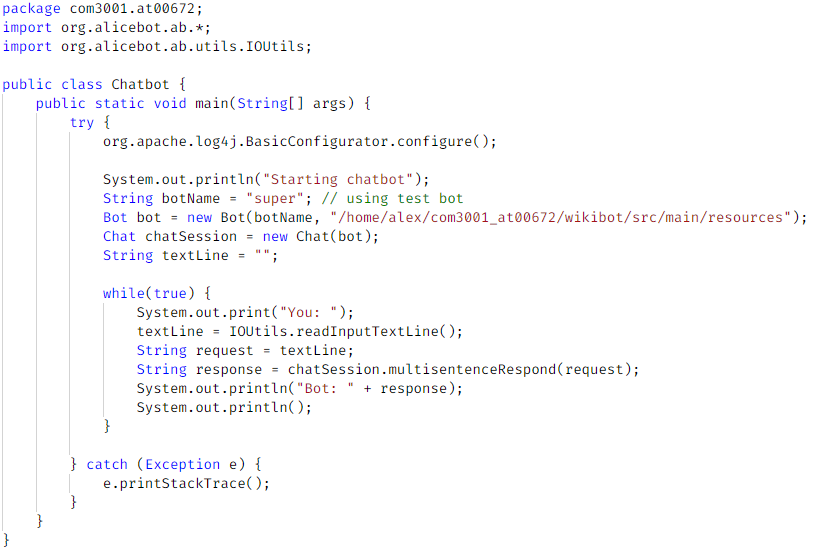
\includegraphics[width=12cm]{code1} }}%
	\qquad
	\subfloat[Chatting with S.U.P.E.R.]{{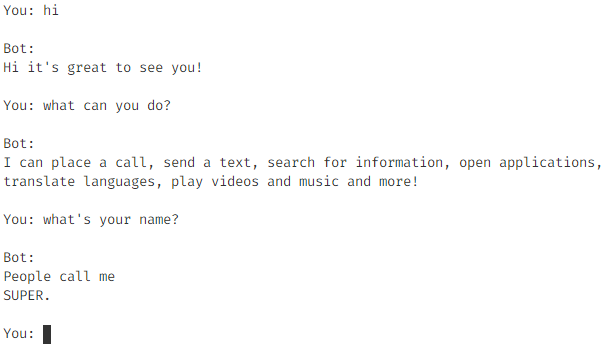
\includegraphics[width=12cm]{super} }}%	
	\caption{Initial chatbot interactions}
	\label{fig:super}
\end{figure}

Having experimented with the example chatbot, the next task was to initialise a new chatbot. The Program AB Bot has a number of functions to load its required files from a directory. The file structure is as follows:

\begin{outline}
	\1 \textbf{bots} The parent bots directory
		\2 \textbf{\emph{botName}} The name of the bot
			\3 \textbf{aiml} The AIML pattern files 
			\3 \textbf{aimlif} AIML Intermediate Format files which are generated by the Bot
			\3 \textbf{config} Configuration files
			\3 \textbf{maps} Map files
			\3 \textbf{sets} Set files
\end{outline}
	
Once the structure was initialised, a file was created named \code{conversation.aiml}, which contained the first AIML patterns for conversing with the chatbot. An excerpt of the contents of this file is shown in Figure~\ref{fig:aiml1}. Some of the key features here are the use for the \code{<srai>} tag on line 17, which is a powerful function for resolving synonyms here. This allows us to route the input of `hi' to the `hello' pattern. This saves us repeating several lines of code, and is used heavily later in the project. Also, in lines 4 and 15 we are using wildcard symbols. This allows us to match zero or more words, and these can then be passed into other parts of the conversation. In AIML, the following wildcards can be used:

\begin{itemize}
	\item \# matches zero or more words (higher priority)
	\item \_ matches one or more words (higher priority)
	\item \^{} matches zero or more words (lower priority)
	\item * matches one or more words (lower priority)
\end{itemize}

So in our `hello' example, the given pattern will match any of the following inputs: {\it{`Hello', `Hello there', `Hi bot', `Hi', `Hi there'}}. It will not, however, match an input such as {\it{`Why hello there'}}, because we have not told the bot how to divide that given input; nor does the bot recognise {\it{`good afternoon'}} and so on.

\begin{figure}[h]
	\centering
	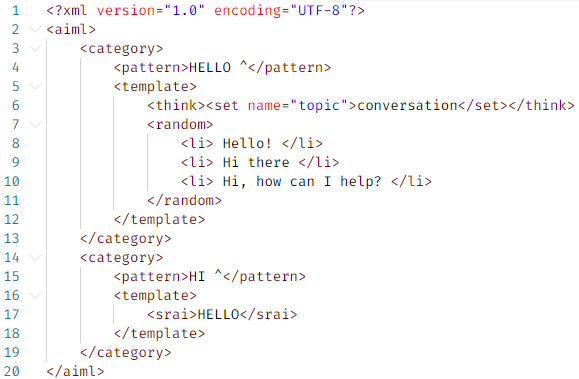
\includegraphics[width=.5\paperwidth]{aiml1}
	\caption{Initial AIML configuration}
	\label{fig:aiml1}
\end{figure}

\subsection{DBPedia}
Now that the basic chatbot system has been set up, we need to provide functionality to the system by querying our datasource. DBPedia was selected based on the research in Section~\ref{sec:dbpedia}, because it provides an organised dataset extracted from Wikipedia articles. It can be queried via a SPARQL endpoint\footnote{http://dbpedia.org/sparql}, and returns data in an RDF format, which can be processed by our system.

There are a number of online resources which allow us to experiment with querying DBPedia. My preferred resource is SPARQL Explorer \footnote{http://dbpedia.org/snorql/}, which allows us to write queries and see the result in several formats, including a tabular format. For example, if we want to find musicians born in Manchester, we can construct the following SPARQL query:
\begin{figure}[h]
	\begin{lstlisting}
		SELECT ?person ?birthPlace ?name
		WHERE {
		  ?person a dbo:MusicalArtist .
		  ?person rdfs:label ?name .
		  ?person dbo:birthPlace ?birthPlace .
		  filter(?birthPlace = dbr:Manchester)
		  filter(langMatches(lang(?name), 'en'))
		} LIMIT 50 
	\end{lstlisting}
	\caption{An example SPARQL query}
	\label{fig:sparql1}
\end{figure}

Executing this query returns a list of the first 50 results of musicians born in Manchester, as shown in Figure~\ref{fig:sparql1}. The format of SPARQL queries has some similarities with SQL queries, using keywords such as \code{SELECT} and \code{WHERE}. In this query, we are filtering to find each person that has the property \code{dbo:MusicalArtist}, which is shorthand for \url{http://dbpedia.org/ontology/MusicalArtist}, which references the DBPedia ontology. We are setting the variable \code{?name} to the property \code{rdfs:label} which contains the name attribute of the person; the same applies for \code{dbo:birthPlace} referencing the birth place attribute. Finally, we are filtering the results; we want the results to only contain musicians whose birth place is Manchester. We also filter the \code{?name} results by language, to remove any duplicate results where the name is given in multiple languages.

\begin{figure}[h]
	\centering
	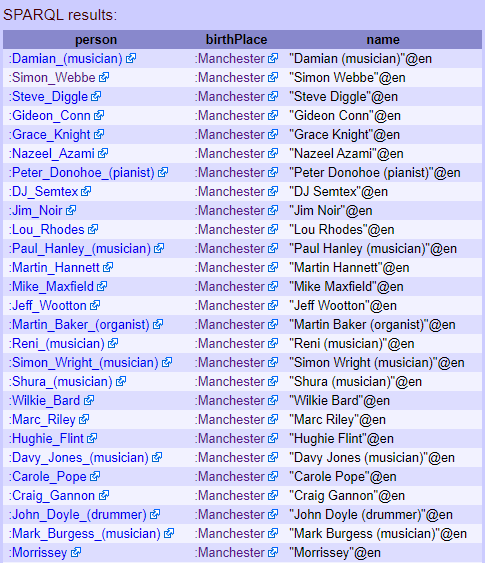
\includegraphics[width=8cm]{snorql}
	\caption{SPARQL query results (truncated)}
	\label{fig:sparql2}
\end{figure}

In our Java system, these queries have to be constructed and executed programmatically, based on the user's input. For executing SPARQL queries, Apache Jena \cite{apachejena} provides RDF functionality for querying an RDF model. To test this, the Apache Jena dependencies are loaded into our Maven dependency file. This allows us to utilise the \code{org.apache.jena} libraries to query the endpoint. To test the connection, a function was written to test the DBPedia endpoint, as shown in Figure~\ref{fig:testrdf}.

\begin{figure}[h]
	\centering
	\subfloat[Test connection code]{{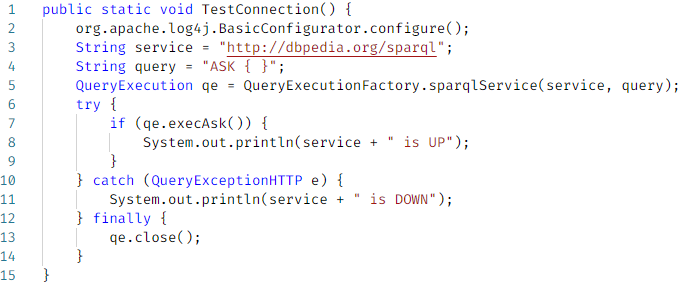
\includegraphics[width=.45\textwidth]{testrdf} }}%
	\qquad
	\subfloat[Successful result]{{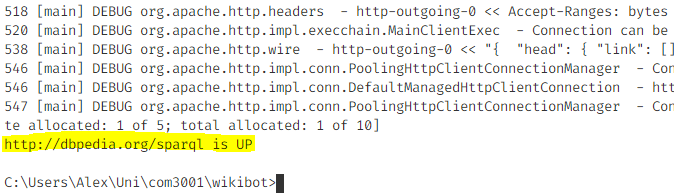
\includegraphics[width=.45\textwidth]{testrdf2} }}%
	\caption{Testing the SPARQL Endpoint}
	\label{fig:testrdf}
\end{figure}

For executing and processing more functional queries, we have to first generate a query string. As an example, we will use the query we saw in Figure~\ref{fig:sparql1}. Once the query has been executed, we have to loop through the results and do some processing, such as printing to the console. The process for this is shown in Figure~\ref{fig:querysparql}. Here, our query string requires the \code{PREFIX} keyword to define the names of the prefixes for the ontologies we are using. The result from this execution exactly matches the result from the experimentation in Figure~\ref{fig:sparql2}.

\begin{figure}[h]
	\centering
	\subfloat[Testing query code]{{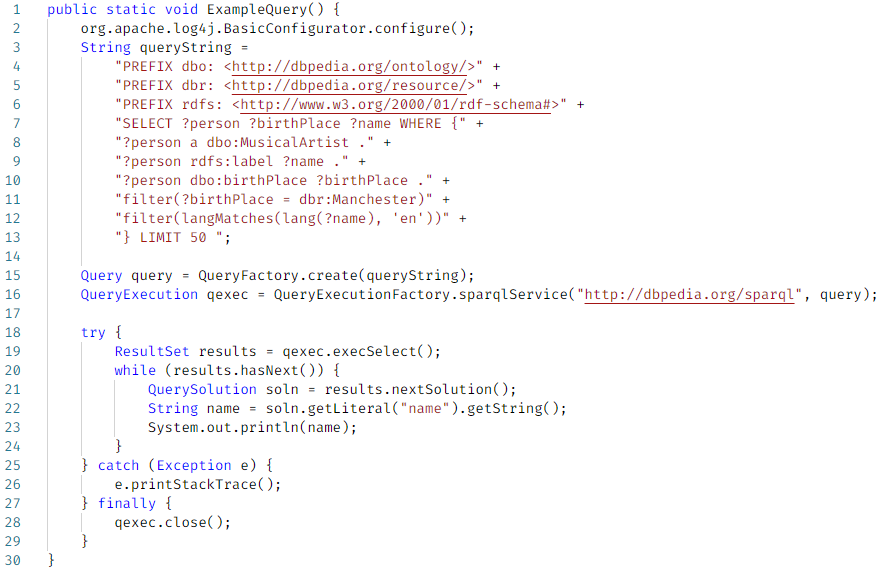
\includegraphics[width=.70\textwidth]{sparql1} }}%
	\qquad
	\subfloat[Result]{{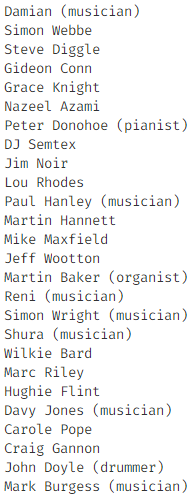
\includegraphics[width=.20\textwidth]{sparql2} }}%
	\caption{Querying the SPARQL endpoint in Java}
	\label{fig:querysparql}
\end{figure}

\subsection{Linking the Chatbot}
Now that we have a basis for querying the DBPedia dataset, the chatbot now has to be able to query the endpoint. For this we need to implement the following functions:
\begin{enumerate}
	\item AIML patterns to match user input to a query
	\item A query builder to convert the user input into a SPARQL query
	\item A service to execute the function and process the results
\end{enumerate}
These functions align with the system architecture design seen previously in Section~\ref{sec:systemdesign}. The next sections explain how these were implemented and connected in the final system to achieve the required functionality.

\subsubsection{AIML Patterns}
One of the key functions of this chatbot is to match input patterns to desired queries. There are a number of challenges that arise here. Firstly, a query can be asked in many different ways. For example, to find out the date of birth of a person, a user may ask: {\it`What is *s birthdate?', `When was * born?', `* birth date', `Tell me when * was born'}. The bot must then distinguish between these queries and {\it`how old is *'} as those are two distinct functions.

Furthermore, one of the requirements of the system is that it can handle pronouns and maintain context. As such, the user should be able to ask follow-up questions by continuing a conversation, e.g. {\it `When was he born?'} - the chatbot must remember who {\it `he'} is, and if that is not known, the chatbot must ask for more information to continue the query.

The AIML patterns become more complex as the system develops to include more functions. For example, Figure~\ref{fig:aiml-comment} shows a fragment of the code for giving a description of a person (Requirement F6). The template uses a number of key features of AIML to achieve the desired functionality.
First, the wildcard (*) is used to match the query value. Next, the \code{<think>} tag allows us to programatically set the {\it{predicates}} of the conversation, which act in essence as variables that can be set and retrieved throughout the conversation. These predicates are used within the \code{ChatbotService} module to process them into a meaningful result.

Line 14 redirects to \code{BOT\_QUERY\_CONTEXT}, the logic for which is shown in Figure~\ref{subfig:aiml1}.
This template determines whether or not a pronoun has been used - {\it{`Who is Alan Turing?'}} versus {\it{`When was he born?'}}. Line 5 uses the \code{<map>} function. Maps can be used to link an input to a result. In this example, our bot has a file named \code{pronouns.txt} in the \code{maps} directory of the bot resources; the contents of which is shown in Figure~\ref{fig:pronouns}. The map simply transforms any pronoun to \code{they}. This means that if a pronoun was used, we determine this conditionally, as in Line 9. If the value of \code{subject} is \code{they}, we then check if the context has been set. If it has, we run the query using the subject that has been previously set. If not, we then ask the user for more information by redirecting to the template shown in Figure~\ref{subfig:aiml2}.

\begin{figure}[h]
	\centering
	\begin{lstlisting}
	he:they
	she:they
	him:they
	her:they
	they:they
	their:they
	\end{lstlisting}
	\caption{Contents of \code{pronouns.txt}}
	\label{fig:pronouns}
\end{figure}

\begin{figure}[pt]
	\centering
	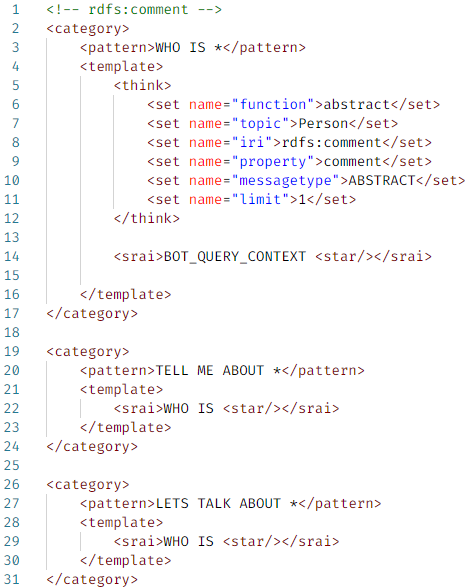
\includegraphics[width=6cm]{aiml-comment}
	\caption{AIML pattern for WHO IS *}
	\label{fig:aiml-comment}
	\subfloat[AIML to decide query context\label{subfig:aiml1}]{{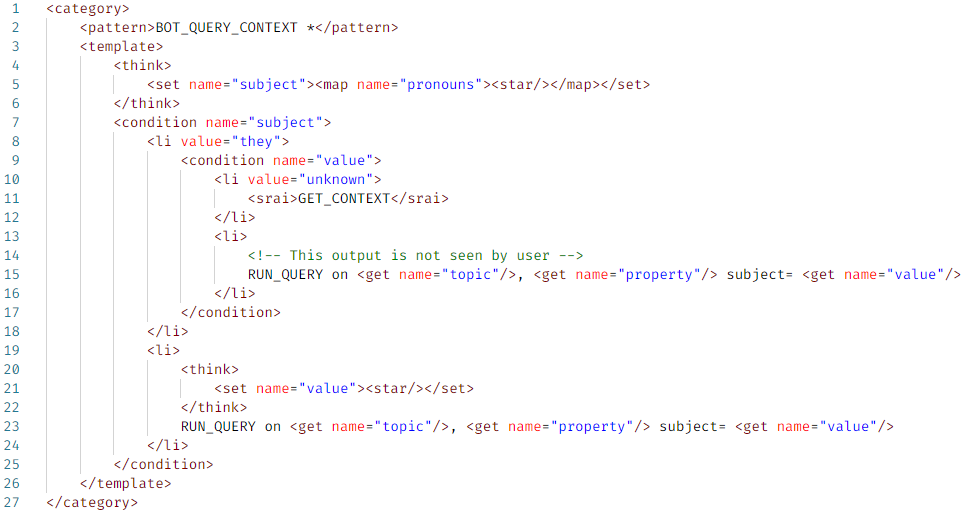
\includegraphics[width=.6\textwidth]{aiml-context} }}%
	\qquad
	\subfloat[AIML to redirect pronominal queries\label{subfig:aiml2}]{{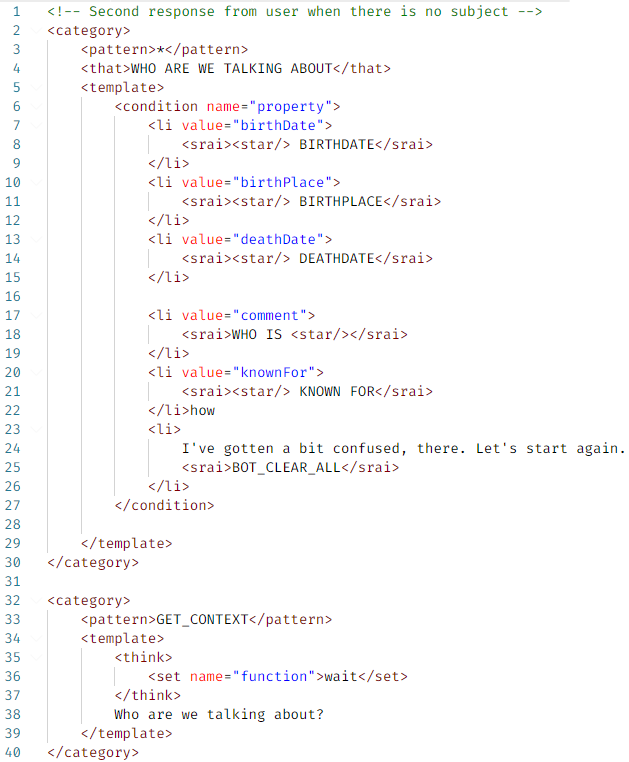
\includegraphics[width=.4\textwidth]{aiml-redirect} }}%
	\caption{AIML logic to handle pronouns}
	\label{fig:aiml-pronouns}
\end{figure}

\newpage
\subsubsection{Query Builder}
We can build a query based on the predicates that we set in the AIML patterns. Most of the simple queries follow a similar pattern to that seen in Figure~\ref{fig:sparql1} - selecting a property given a set of conditions. For these queries we can build a query string, inserting the values provided by the user from the AIML predicates.

In the final system, an instance of the UserQuery class is used to maintain the attributes of the user's query. We store the predicates in a \code{HashMap}, which are retrieved from the \code{alicebot.ab.Chat} instance. We can then make decisions about how the query is built in the \code{QueryBuilder} class. Based on these predicates, the \code{QueryBuilder} can construct an appropriate query for the \code{DBPedia} service to execute. One of the issues for future extension of the project is that some queries must have separate methods for execution. For example, a list query has to be generated and executed differently from an abstract query. The final solution has been developed to handle the queries established in the requirements, but adding further features would require manually adding AIML patterns and query functions - this drawback is discussed at length in Chapter~\ref{ch:conclusion}.

\subsubsection{DBPedia Service}
The role of the \code{DBPedia} class is to execute queries and return a result. This class is divided into a number of methods for each type of query. For example, executing a query about a person in \code{executePersonQuery()} requires different logic to \code{executeAgeQuery()} where further processing has to take place. Each method makes changes to the \code{Message} instance which contains the chatbot's response. The \code{Message} object has a number of attributes relating to the content and information stored in the message. It also has a list of \code{MessageItems}, where a \code{Message} may contain a list of multiple items. The information stored here is processed by the web interface in order to display the information in the correct format, as discussed in the next section.

\subsection{Web Interface}
Spring Boot \cite{springmanual} was used in this project has the web framework, mainly because of its popularity and configurability for web-based Java projects. To initalise this, the required dependencies are added to the project's \code{pom.xml} file. The \code{org.springframework.boot} provides many helper classes for configuring a Spring Boot application.

In order to manage the web application, our \code{WebController} routes requests and manages state. The web application routing is simple, because there are only three mappings to deal with:
\begin{itemize}
	\item GET index: Displays all messages between user and bot
	\item POST submitMessage: User sends a new message to the bot
	\item POST clear: Clears the chat history
\end{itemize}

For displaying the web views, Thymeleaf \footnote{https://www.thymeleaf.org/} is used in this project because it integrates well with Spring, and gives us a lot of flexibility with conditionally styling and displaying elements. Bootstrap \footnote{https://getbootstrap.com/} is also used as a CSS library to homogenize the front-end design, and allow for quickly configuring elements.

The final user interface is shown in Figure~\ref{fig:final-ui}. The layout is simple, with a \code{navbar} element at the top and the main body containing the chat window, which contains the messages sent between the user and the bot. The messages are retrieved from the \code{MessageRepository} by the controller, which are iterated over by the Thymeleaf function in the \code{index.html} page. These messages are conditionally formatted, based on the \code{Sender} attribute of the message. We can see that the larger message is formatted to contain an image and a link - this is based on the \code{MessageType} attribute being equal to \code{ABSTRACT} - this was initially flagged by the bot AIML pattern when the user entered the query {\it`who is alan turing'}.

\begin{figure}[h]
	\centering
	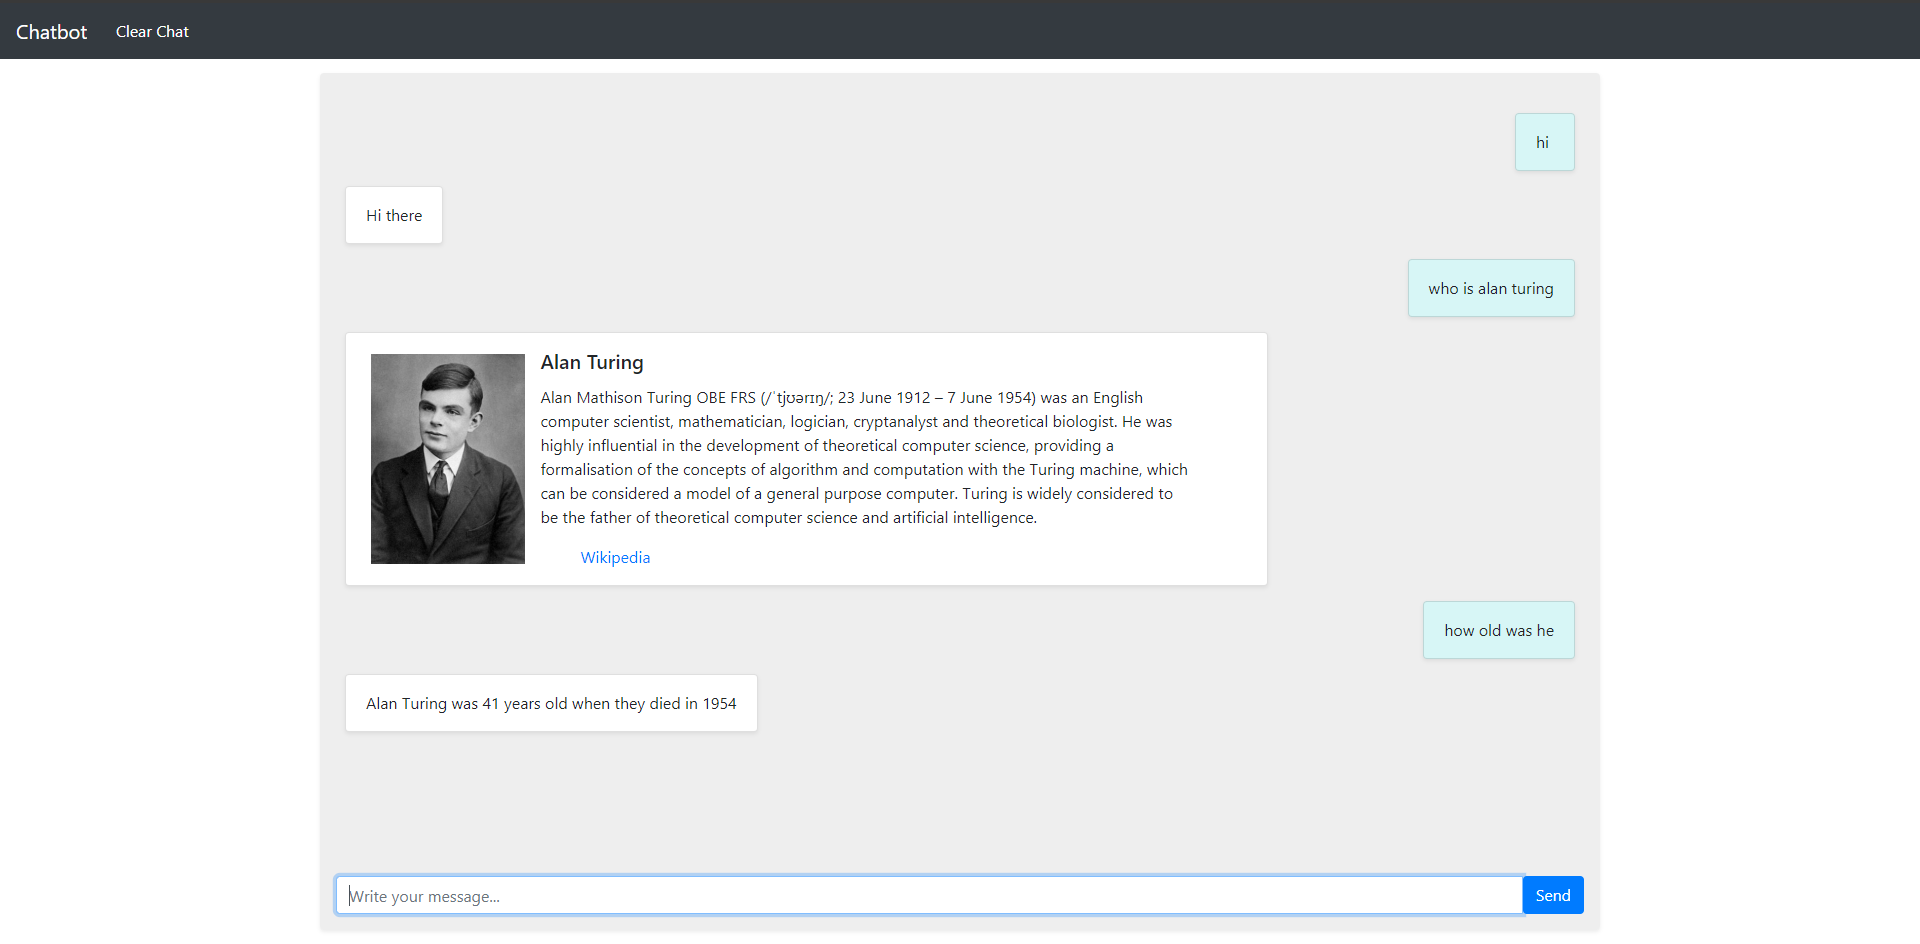
\includegraphics[width=\textwidth]{final-ui}
	\caption{Final UI design}
	\label{fig:final-ui}
\end{figure}

\newpage
\subsection{Hibernate Database}
In order to maintain a conversation history with the chatbot, as well as manage multiple users, a database is required to store messages. However, storing user data has legal and ethical considerations - this is discussed in detail in Chapter~\ref{ch:ethics}. For this implementation, I made a conscious effort to store as little information about the user as possible. Hibernate H2 \footnote{http://www.h2database.com/html/main.html} allows us to persist data in our web application, as well as provide object-relational mapping (ORM) between the objects and the database. H2 allows us to create an in-memory database, so that data is not stored on the disk and is lost when the application is restarted.

The schema of the database is automatically generated on start-up, based on the Spring \code{Entities} in our application. For this application we have the \code{Message} entity, which stores the content and metadata of each message. We also have the \code{MessageItem} entity, which can form the basis of a \code{LIST} message, where each \code{MessageItem} may have metadata such as a URI. In the \code{Message} entity, we define the relationship between \code{Message} and \code{MessageItem} as \code{OneToMany}, as we can have multiple \code{MessageItems} in a single \code{Message}. The attributes of \code{Message} are shown in Figure~\ref{fig:message}, which shows the tags used to achieve this objective.

\begin{figure}[h]
	\centering
	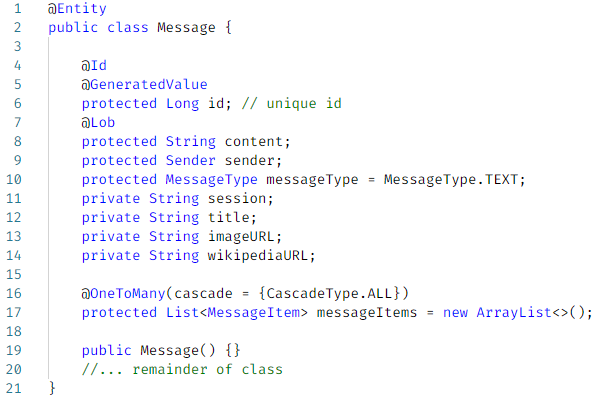
\includegraphics[width=.5\textwidth]{message}
	\caption{Message class}
	\label{fig:message}
\end{figure}


Spring Data provides CRUD operations (create, read, update, delete) for the ORM using a repository interface; here we are using \code{CrudRepository}. This allows us to easily add messages to the conversation. This interface is provided by the \code{MessageRepository} class - a similar one is required for \code{MessageItemRepository} to provide an interface for the \code{MessageItem} entities. The \code{MessageRepository} interface provides functionality to the \code{WebController}, including adding additional functions such as finding messages by Session ID. The code for this is shown in Figure~\ref{subfig:message}, and is used in Figure~\ref{subfig:webcontroller} to save messages to the database.

\begin{figure}[h]
	\centering
	\subfloat[MessageRepository interface \label{subfig:message}]{{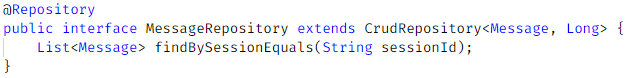
\includegraphics[width=.6\textwidth]{messagerepo} }}%
	\qquad
	\subfloat[WebController logic \label{subfig:webcontroller}]{{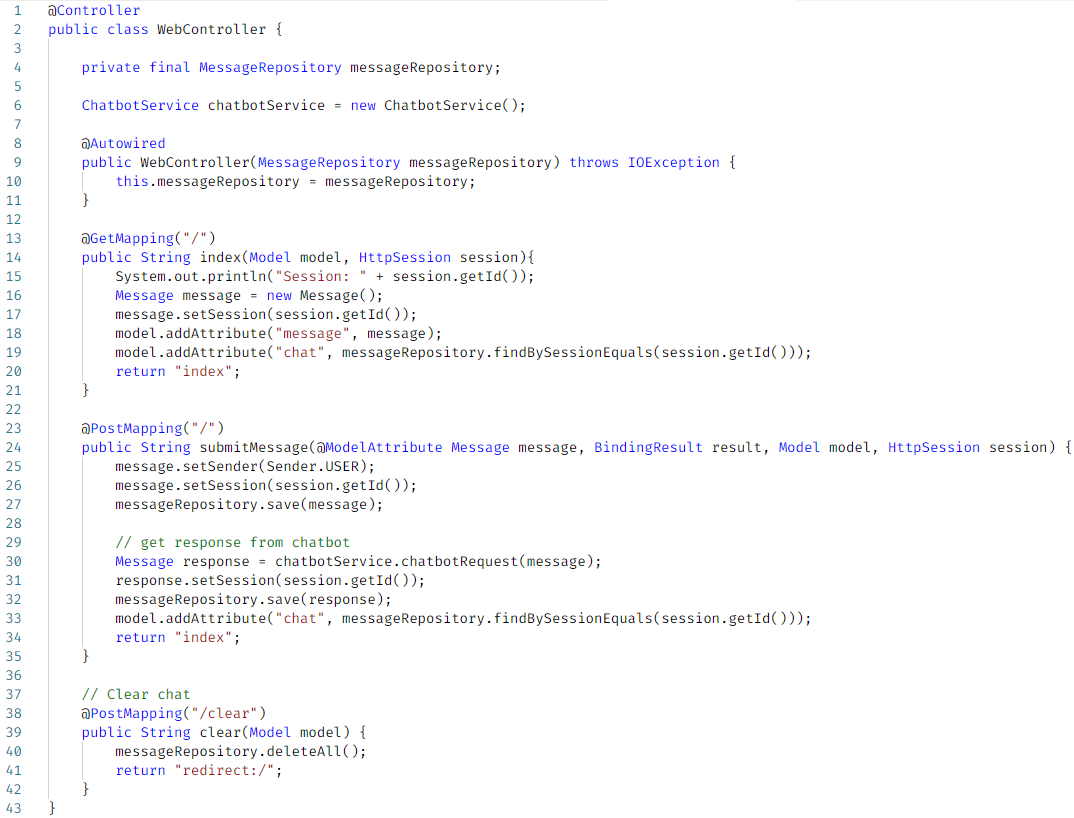
\includegraphics[width=\textwidth]{webcontroller} }}%
	\caption{Controller logic}
	\label{fig:controller}
\end{figure}

\newpage
\section{Additional Queries}
Once the initial system had been implemented, it became clear that adding additional queries for attributes was trivial. For example, the query pattern seen in Figure~\ref{fig:aiml1}, which queries \code{rdfs:label} could be easily replicated for the remaining attributes in the requirements specification. This allowed us to easily add additional queries beyond the scope of the requirements. As such, additional functions were added that could be useful for the user which were not identified in the specification. These include:
\begin{itemize}
	\item Person known for
	\item Person influences
	\item Person influenced by
\end{itemize}
Although this contradicts the scope of the project outlined in the specification and Section~\ref{sec:scope}, I believe these extensions provide a more complete final implementation, and act as a proof-of-concept for future development of the system.


\section{Challenges}
This section discusses some of the challenges encountered during the implementation of this project. It describes some of the solutions used to overcome these obstacles.

\subsection{Limitations of AIML}
One of the fundamental challenges of using the pattern-based AIML is handling synonyms. I discovered that there are many ways that a particular question can be asked. Furthermore, since the requirements of the system pertain to both Person queries and Country queries, the system must be able to distinguish between the two topics of conversation.

The use of sets and maps was key to solving this problem. In order to `teach' the chatbot what a country is, a set was created named \code{countries.txt} with a list of every country from the DBPedia dataset. These were loaded programatically using a DBPedia query in the \code{ChatbotUtils} class. One issue here was that simply querying a list of all records belonging to \code{dbo:Country} also included every historic kingdom, dominion, dynasty, caliphate, as well as some bizarre outliers - a further discussion of inconsistencies of the dataset is given in Section~\ref{sec:dataset}. Therefore, to return valid data, the results had to be filtered to exclude records with a \code{dbo:dissolutionYear}, as well as include countries that had a \code{dbo:Capital}.

The final query used in this function is given in Figure~\ref{fig:sparqlcountry}. Given a list of all countries, we can then map the country to its Uniform Resource Locator (URI) to easily query that exact country - this is handled in the file \code{country2dbr.txt}.

\begin{figure}[h]
	\begin{lstlisting}
		SELECT DISTINCT ?country ?name
		WHERE {
		  ?country a dbo:Country.
		  ?country dbo:capital ?capital .
		  ?country rdfs:label ?name 
		  FILTER NOT EXISTS { ?country dbo:dissolutionYear ?yearEnd }
		  FILTER langMatches(lang(?name), 'en')
		} ORDER BY ?country
	\end{lstlisting}
	\caption{SPARQL for listing every country}
	\label{fig:sparqlcountry}
\end{figure}


\subsection{SPARQL Queries}
One of the challenges with querying the DBPedia dataset arises from the requirement for generating lists (requirement F17). While it is trivial to list every actor using a basic query, it is important to return meaningful results to the user. For example, if the user wants a list of actors, we might use the query shown in Figure~\ref{subfig:unranked}. The challenge here is: what order should these results be displayed? If they are displayed alphabetically, as shown in Figure~\ref{subfig:unrankedresults}, the user will not get much use out of those results, especially because named beginning with special characters such as brackets are shown first.

The solution here was to use a computed PageRank \cite{rank2014}. These PageRank scores can be integrated into our query using the vRank implementation by \citet{rank2012} to provide a numerical PageRank value for DBPedia resources. The query and results are shown in Figure~\ref{fig:ranked}, which provides considerably more `useful' responses because the highest ranked results are shown first.

\newsavebox\unrankbox
\begin{lrbox}{\unrankbox}
	\begin{lstlisting}
		SELECT * WHERE {
		?person a dbo:Actor .
		?person foaf:name ?name .
		} ORDER BY ASC(?name)
		LIMIT 10
	\end{lstlisting}
\end{lrbox}

\begin{figure}[p]
	\centering
	\subfloat[SPARQL query for sorted list \label{subfig:unranked}]{\usebox\unrankbox} \qquad
	\subfloat[Results of query \label{subfig:unrankedresults}]{{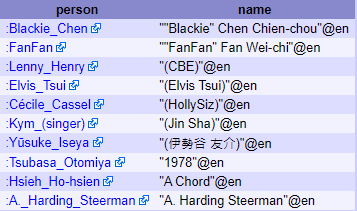
\includegraphics[width=.4\textwidth, valign=m]{vrank1} }}
	\caption{Ordering a list alphabetically}
	\label{fig:unranked}
\end{figure}

\newsavebox\rankbox
\begin{lrbox}{\rankbox}
	\begin{lstlisting}
		PREFIX vrank:<http://purl.org/voc/vrank#>
		SELECT DISTINCT ?person ?v
		FROM <http://dbpedia.org>
		FROM <http://people.aifb.kit.edu/ath/#DBpedia_PageRank>
		WHERE {
		?person a dbo:Actor .
		?person foaf:name ?name .
		?person vrank:hasRank/vrank:rankValue ?v .
		} ORDER BY DESC(?v)
		LIMIT 10
	\end{lstlisting}
\end{lrbox}

\begin{figure}[p]
	\centering
	\subfloat[SPARQL query for ranked list \label{subfig:ranked}]{\usebox\rankbox} \qquad
	\subfloat[Results of query \label{subfig:rankedresults}]{{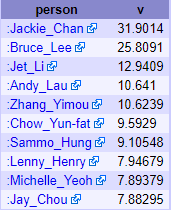
\includegraphics[width=.25\textwidth, valign=m]{vrank2} }}
	\caption{Ordering a list by PageRank}
	\label{fig:ranked}
\end{figure}

\subsection{Dataset Inconsistencies}
\label{sec:dataset}
One of the challenges I encountered working with DBPedia is inconsistencies in the dataset. For example, when working with the Country ontology, one of the tasks was to extract a list of all countries. While testing this function, however, England was not appearing in the list. Upon investigation, this was caused by an error in the dataset - the England resource was flagged as belonging to the \code{MusicalArtist} ontology as opposed to the \code{Country} ontology (Figure~\ref{fig:england}).

The quick-fix solution here was to simply add this value manually to the list of known countries. However, it highlighted the importance of understanding the drawbacks of an automated, community-drived project. More robust solutions for the future may be to select countries by a different condition, but again there are some shortcomings here. For example, member states of the United Nations (\code{yago:WikicatMemberStatesOfTheUnitedNations}) would group England under United Kingdom. The YAGO\footnote{https://github.com/yago-naga/yago3} Country ontology contains England, but also many historical kingdoms and counties. This led to the distinction between a {\it country} and a {\it sovereign state} and how each is defined \cite{fowler1996}; however, geopolitics is beyond the scope of this chatbot project.

\begin{figure}[p]
	\centering
	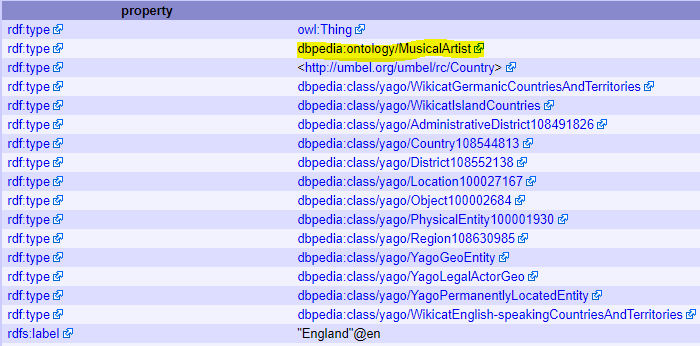
\includegraphics[width=.5\textwidth]{england}
	\caption{Inconsistency with England resource}
	\label{fig:england}
\end{figure}

\section{Conclusion}
Overall, the implementation phase of this project was broadly successful. Some phases were easier than expected and did not take as much time as expected in the plan, such as initialising the chatbot. Also, once the system for answering one query was implemented, it was simple to extend this to many other queries. However, being able to distinguish query topics between people and countries did provide a challenge, and the solution for this is not without issue. In the next chapter we test the entire system to determine how effective it is, and whether the users accept it as a working, valid system.

